\documentclass[9pt,twocolumn,twoside]{../../styles/osajnl}
\usepackage{fancyvrb}
\usepackage[colorinlistoftodos,prependcaption,textsize=normal]{todonotes}
\journal{i524} 

\title{Deployment Model of Juju}

\author[1,*]{Sunanda Unni}

\affil[1]{School of Informatics and Computing, Bloomington, IN 47408, U.S.A.}
\affil[*]{Corresponding authors: suunni@indiana.edu}

\dates{paper2, \today}

\ociscodes{Cloud, I524, Juju, IaaS}

% replace this with your url in github/gitlab
\doi{\url{https://github.com/cloudmesh/sp17-i524/raw/master/paper2/S17-IO-3022/report.pdf}}


\begin{abstract}
Developing an application for the cloud is accomplished by relying on
the Infrastructure as a Service (IaaS) or the Platform as a Service
(PaaS).  Juju is a software from Canonical that provides open source
service orchestration using a model of IaaS. Juju charms can be
deployed for IaaS on cloud services such as Amazon Web Services (AWS),
Microsoft Azure and OpenStack. Deep Server provisioning is provided by
Juju using MAAS, Metal as a Service. We are exploring the deployment
model of Juju.
\end{abstract}

\setboolean{displaycopyright}{true}

\begin{document}

\maketitle

\TODO{This review document is provided for you to achieve your
  best. We have listed a number of obvious opportunities for
  improvement. When improving it, please keep this copy untouched and
  instead focus on improving report.tex. The review does not include
  all possible improvement suggestions and if you sea comment you may
  want to check if this comment applies elsewhere in the document.}
\TODO{Abstract: When writing you should be careful to be gender specific pronouns, such as HE. Also, please check spelling on ecosystem}



\section{Introduction}
Deploying software component systems \cite{lascu2015automatic} is
becoming a critical challenge, especially due to the advent of Cloud
Computing\SE technologies that make it possible to quickly run complex
distributed software systems on-demand on a virtualized infrastructure
at a fraction of the cost compared to a few years ago. When the number
of software components needed to run the application grows,\GE and their
interdependencies become too complex to be manually managed, it is
important for the system administrator to use high-level languages for
specifying the expected minimal system.

\TODO{Introduction: provide lowercase lettering for cloud computing. Please remove comma after grows}


\section{IaaS, PaaS and MaaS}
The IaaS provides a set of low-level resources forming a bare
computing environment. Developers pack the whole software stack into
virtual machines containing the application and its dependencies and
run them on physical machines of the provider's cloud. Exploiting the
IaaS directly allows a great flexibility but requires also a great
expertise and knowledge of the cloud and application entities involved
in the process IaaS describes the provision of processing, storage and
networking (and potentially) other basic computing resources, over a
network and in an on-demand fashion. An example of IaaS is the
AWS\cite{www-aws}, Juju.

IaaS customers does not host or manage the dedicated or virtual
server. Figure \ref{fig:juju-scheme-of-work-yurkevich} for Juju
scheme of work as IaaS.

\begin{figure}[htbp]
  \centering
  \fbox{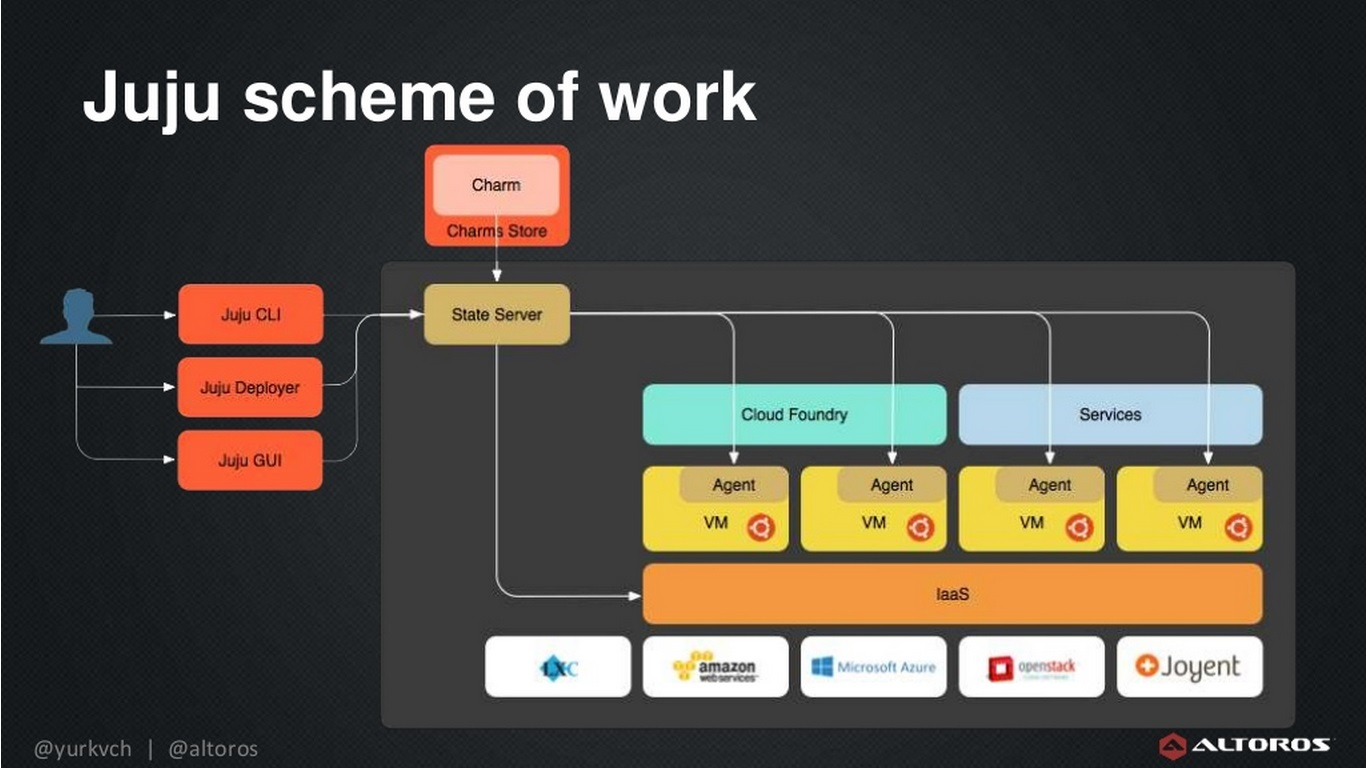
\includegraphics[width=\linewidth]{images/juju-scheme-of-work-yurkevich.jpg}}
  \caption{Basic Deployment of Juju scheme of work.}
  \label{fig:juju-scheme-of-work-yurkevich}
\end{figure}


In PaaS (e.g., Google App Engine \cite{www-googleappengine}, Azure
\cite{www-azure}) a full development environment is
provided. Applications are directly written in a programming language
supported by the framework offered by the provider, and then
automatically deployed to the cloud. The high-level of automation
comes however at the price of flexibility: the choice of the
programming language to use is restricted to the ones supported by the
PaaS provider, and the application code must conform to specific APIs.

\section{Juju}

In the IaaS, two deployment approaches \cite{lascu2015automatic} are
gaining more and more momentum: the holistic and the DevOps one.  In
the former, also known as model-driven approach, one derives a
complete model for the entire application and the deployment plan is
then derived in a top-down manner. In the latter, put forward by the
DevOps community \cite{www-devOps}, an application is deployed by
assembling available components that serve as the basic building
blocks. This emerging approach works in a bottom-up direction: from
individual component descriptions and recipes for installing them, an
application is built as a composition of these recipes.

One of the representative for the DevOps approach is Juju
\cite{www-juju}, by Canonical. It is based on the concept of charm:
the atomic unit containing a description of a component.

In 2.0, Juju follows a Controller-Model type of configuration. A Juju
controller is the management node of a Juju cloud environment. In
particluar\SE, it houses the database and keeps track of all the models
in that environment. Although it is a special node, it is a machine
that gets created by Juju (during the "bootstrap" stage) and, in that
sense, is similar to other Juju machines.

A Juju model is an environment associated with a controller. During
controller creation two models are also created, the 'controller'
model and the 'default' model. The primary purpose of the 'controller'
model is to run and manage the Juju API server and the underlying
database. Additional models may be created by the user.

Since a controller can host multiple models, the destruction of a
controller must be done with ample consideration since all its models
will be destroyed along with it.

\TODO{Please correct the spelling error listed.}
\section{Juju Installation}
Installing Juju is straight forward, it is described in detail in
Getting Started document \cite{www-jujucharm-documentation} and Paper
regarding deploying Juju on MaaS \cite{juju-paper}.

The command to install Juju is shown in Fig \ref{fig:juju-install}.
\begin{figure}
  \centering
  \caption{Juju installation steps\cite{www-juju}}\label{fig:juju-install}
  \begin{quote}
    \begin{Verbatim}
$ sudo apt-get update && sudo apt-get install juju
    \end{Verbatim}
  \end{quote}
\end{figure}

Not covering setup of LXD or MaaS for the physical containers or
cluster on which Juju is to be installed. We can refer to
\cite{www-jujucharm-documentation} for LXD and \cite{juju-paper} for
MaaS installation.

To create a controller, juju bootstrap command is used. Two ways to bootstrap
\begin{itemize}
  \item[1.] Generate config with the environment specified in yaml, as
    shown in Fig \ref{fig:bootstrap}.
  \item[2.] By specifying the details on command line as shown in Fig
    \ref{fig:bootstrapcmd}.
\end{itemize}

\begin{figure}
  \centering
  \caption{Juju bootstrap command with yaml configuration set \cite{www-juju}.}
  \label{fig:bootstrap}
  \begin{quote}
    \begin{Verbatim}
$ sudo juju generate-config
$ edit the environments.yaml file
$ sudo juju sync-tools
$ sudo juju bootstrap
    \end{Verbatim}
  \end{quote}
\end{figure}

\begin{figure}
  \caption{Juju bootstrap command with command line settings \cite{www-juju}.}
  \label{fig:bootstrapcmd}
  \begin{quote}
    \begin{Verbatim}
$ sudo juju bootstrap localhost lxd-test

lxd-test is the controller on the local machine.
    \end{Verbatim}
  \end{quote}
\end{figure}

\TODO{It may be helpful to define LXD }

\section{Installation of Charms}
Fig \ref{fig:charms-bundles-2x} shows the deployment model of Charms.

\begin{figure}[htbp]
  \centering
  \fbox{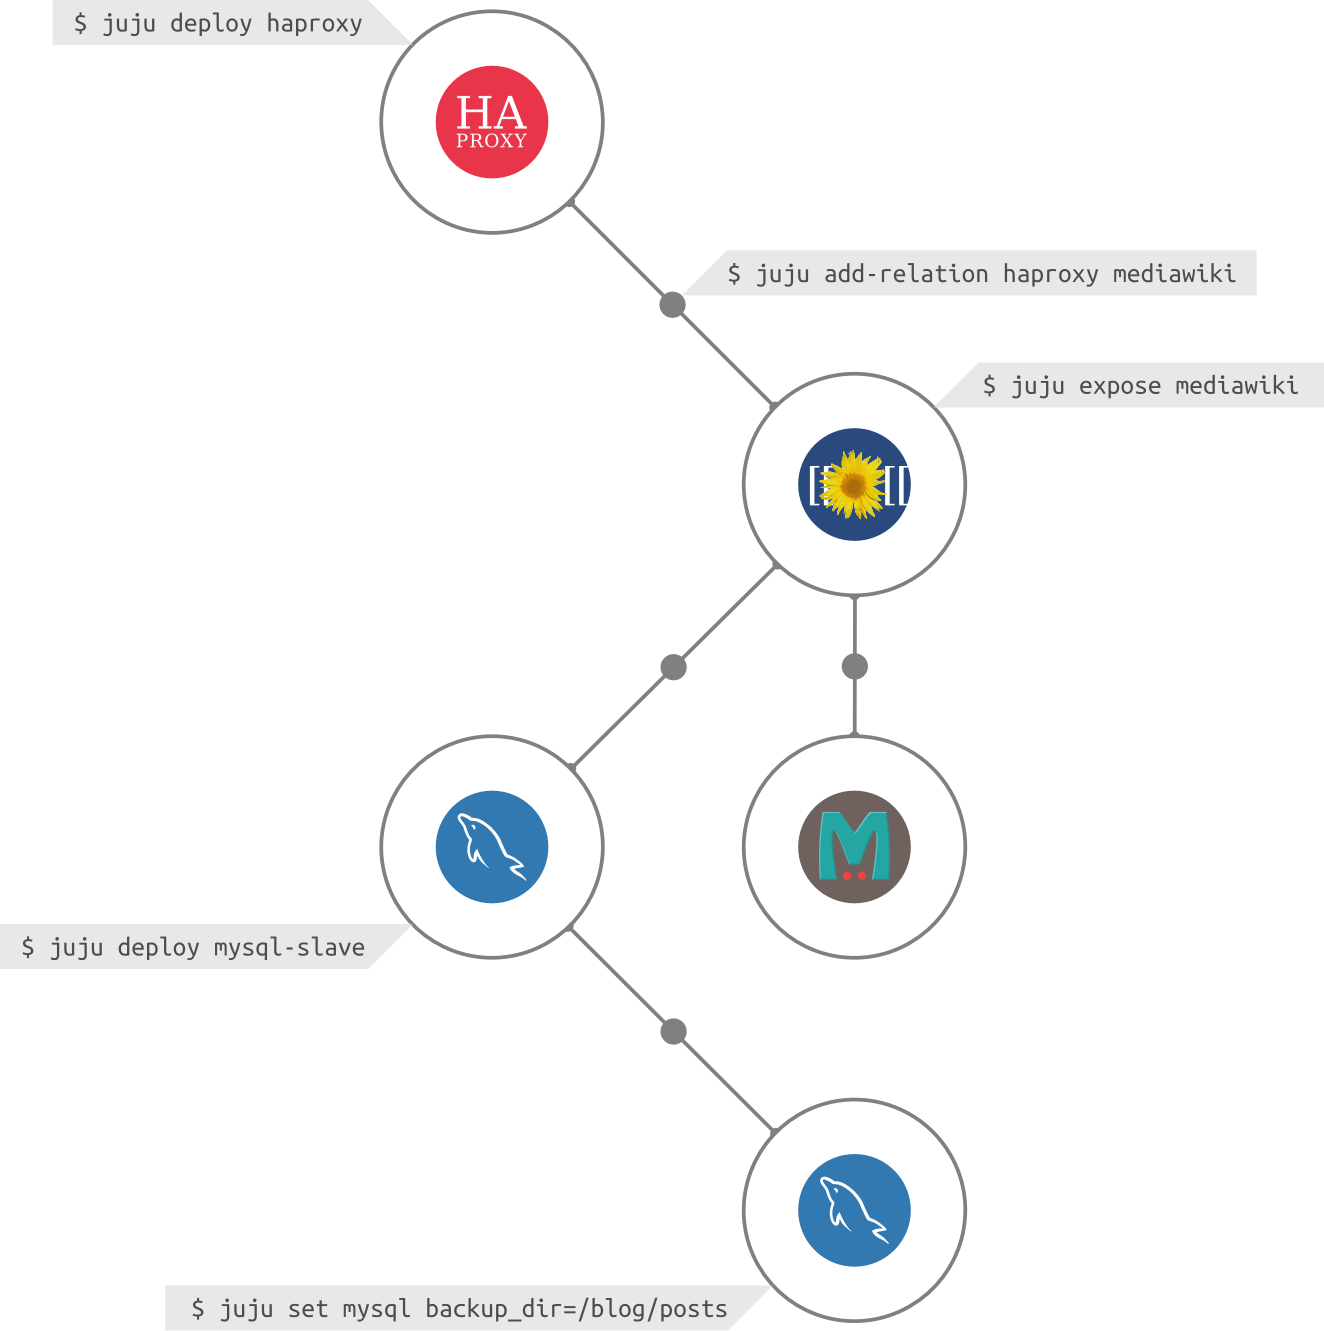
\includegraphics[width=\linewidth]{images/charms-bundles-2x.png}}
  \caption{Charms and Bundles \cite{www-juju}.}
  \label{fig:charms-bundles-2x}
\end{figure}

When deploying charms you can do the following-
\begin{itemize}
\item[1.] Download them from external repositories as you deploy. For
  direct installation from external repository, we can use Fig
  \ref{fig:charm-deploy}.

\item[2.] Download them first to a local repository and then point to
  the repository as you deploy. For deploying from local repository
  you can install bazar as shown in Fig \ref{fig:charm-deploy-local}.
  
\end{itemize}


\begin{figure}
  \caption{Juju Charm deploy from external repository \cite{www-juju}.}
  \label{fig:charm-deploy}
  \begin{quote}
    \begin{Verbatim}
$ sudo apt-get install charm-tools
$ charm get <charm>
$ juju deploy local:trusty/<charm-name>
    \end{Verbatim}
  \end{quote}
\end{figure}


\begin{figure}
  \caption{Juju Charm deploy from local repository \cite{juju-paper}.}
  \label{fig:charm-deploy-local}
  \begin{quote}
    \begin{Verbatim}
$ sudo apt-get install bzr
$ mkdir -p /opt/charms/trusty; cd /opt/charms/trusty
$ bzr branch lp:charms/<charm-name>
$ juju deploy repository=/opt/charms local:trusty/<charm-name>
    \end{Verbatim}
  \end{quote}
\end{figure}


Status of installation can be checked by command as shown in Fig
\ref{fig:deploy-status}.
\begin{figure}
  \caption{Juju Charm installation status \cite{www-juju}.}
  \label{fig:deploy-status}
  \begin{quote}
    \begin{Verbatim}
$ juju status
    \end{Verbatim}
  \end{quote}
\end{figure}

On successful installation of MySQL and mediawiki, we can see the status
as shown in Fig \ref{fig:juju-mediawiki-status}.

\begin{figure}[htbp]
\centering
\fbox{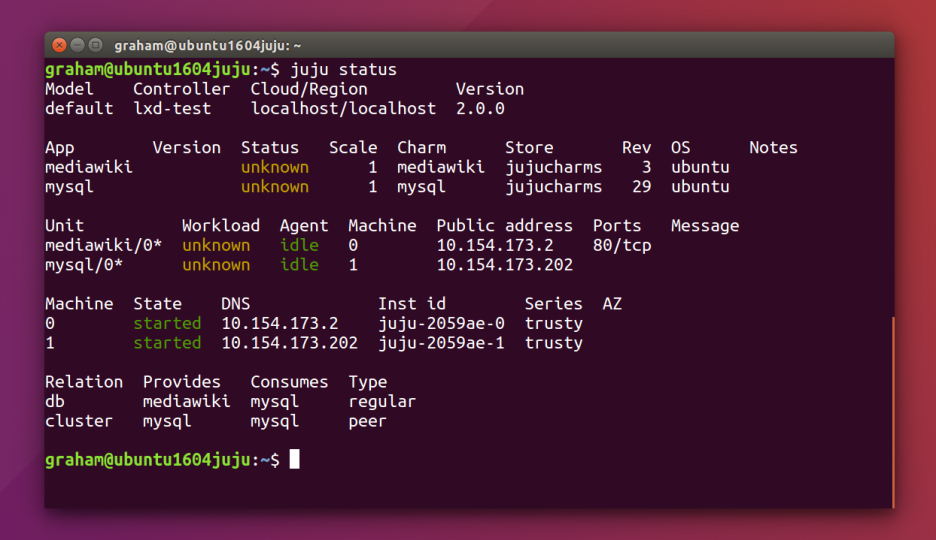
\includegraphics[width=\linewidth]{images/juju-mediawiki-status.png}}
\caption{Juju status post installation of Bundle
  \cite{www-jujucharm-documentation}.}
\label{fig:juju-mediawiki-status}
\end{figure}

\TODO{The graph is difficult to read and not sure if it contributes to an additional understanding of the paper}
\section{Bundling}
A Bundle is an encapsulation of complex deployments including many
different applications and connections.
Bundles are deployed as-
\begin{itemize}
\item[1.] From the Juju Charm Store as shown in Fig
  \ref{fig:deploybundle-status}.
\begin{figure}
  \caption{Deploy bundle from Juju Charm Store
    \cite{www-jujucharm-documentation}.}
  \label{fig:deploybundle-status}
  \begin{quote}
    \begin{Verbatim}
juju deploy cs:bundle/wiki-simple-0
    \end{Verbatim}
  \end{quote}
\end{figure}
    
\item[2.] By exporting the current configuration into a
  bundle. Juju-UI can be used for exporting the current configuration
\end{itemize}

\section{Advantages of Juju}

Scaling the setup is possible. No prior knowledge of application stack
required. Charm store provides charms for a lot of common Opensource
applications. Bundling helps in easy re-deployment to new environment.
Juju works with the exiting Configuration management tool.

\section{Drawbacks of Juju}

In order to use Juju, some advanced knowledge of the application to
install is mandatory. This is due to the fact that the metadata does
not specify the required functionalities needed by a component.
Currently Juju can be used for deployments on limited OS - Windows,
CentOS, and support for Ubuntu. Juju does not still support handling
of circular dependencies


\section{Conclusion}
For Application provisioning Juju does provides orchestration similar
to Puppet, Chef, Salt etc. Advantage is Juju comes with GUI in open
source version and is interoperable with most of the major cloud
providers.

\bibliography{references}
 
\end{document}
